\documentclass[12pt,a4paper]{book}
% 使用ctex包以支持中文
\usepackage{ctex}

% 设置页边距
\usepackage[a4paper, left=2.5cm, right=2.5cm, top=2.5cm, bottom=2.5cm]{geometry}

% 引入amsmath宏包用于数学环境
\usepackage{amsmath}
\usepackage{amsfonts}
\usepackage{amssymb}

\usepackage{tikz}
\usetikzlibrary{positioning,calc}

% 为图表等浮动体添加更友好的支持
\usepackage{graphicx}
\usepackage{float}
\usepackage{makeidx}
\makeindex
% 设置超链接
\usepackage{hyperref}
\hypersetup{
    colorlinks=true,
    linkcolor=blue,
    filecolor=magenta,      
    urlcolor=cyan,
}

% 自定义页眉页脚
\usepackage{fancyhdr}
\pagestyle{fancy}
\fancyhf{}
\rhead{\leftmark}
\lhead{\rightmark}
\rfoot{\thepage}

% 设置目录深度
\setcounter{secnumdepth}{2} % 编号到 section(即章、节、小节都编号)
\setcounter{tocdepth}{1}    % 目录只显示到 section 层级

\begin{document}

% 封面
\begin{titlepage}
\centering
\vspace*{5cm}
{\Huge 凸优化学习笔记}\\[2cm]
{\LARGE 陈皞翰 Chen Haohan}\\[2cm]
{\large 最后修改日期:\today}
\end{titlepage}
\let\cleardoublepage\clearpage

% 目录
\tableofcontents

% 前言
\chapter*{前言}
\addcontentsline{toc}{chapter}{前言}
本篇笔记为本人学习斯坦福大学EE364a课程的记录,内容包括凸优化的基本概念、定理及其证明等,主要是自己学习过程的记录,也希望能对同样学习这门课程的同学有帮助。

参考书籍:Convex Optimization by Stephen Boyd and Lieven Vandenberghe


% 正文开始
\mainmatter
\part{基础知识}
\chapter{课程导入}
本章主要给出数学优化问题的概览,并且着重介绍凸优化的相关知识。在本课程中,我们将会学习如何高效可靠的解决凸优化问题,并且解决一些实例。
\section{数学优化概述}
一般数学优化问题的标准形式为:
\begin{align*}
\text{minimize(使最小化)} \quad & f_0(x) \\
\text{subject to(满足)} \quad & f_i(x) \leq 0, \quad i = 1, \ldots, m \\
& g_i(x) = 0, \quad i = 1, \ldots, p
\end{align*}
(这里教材上可能有误,没有等式约束)其中$x$是$\mathbb{R}^n$上的向量,为该优化问题的优化(决策)变量;$f_0$是$\mathbb{R}^n \rightarrow \mathbb{R}$上的函数,为目标函数;$f_i(x)$是$\mathbb{R}^n \rightarrow \mathbb{R}$上的函数,为不等式约束($b_i$为该不等式的限制);$g_i(x)$是$\mathbb{R}^n \rightarrow \mathbb{R}$上的函数,为等式约束。
这个优化问题表达的就是:在满足所有约束的前提下,找到一个$x$使得目标函数$f_0(x)$最小。

如果一个优化问题中的目标函数以及所有不等式约束均为线性的,那么称该问题为线性优化问题。也就是所有$f_i$满足如下条件:$$f_i(\alpha x + \beta y) = \alpha f_i(x) + \beta f_i(y) , \quad i = 0, 1, \ldots, m,\quad \forall \alpha, \beta \in \mathbb{R} ,\quad \forall x, y \in \mathbb{R}^n $$

本课程主要介绍凸优化问题,凸优化问题要求目标函数和所有不等式约束均为凸函数,即:
$$f_i(\alpha x + \beta y) = \alpha f_i(x) + \beta f_i(y) , \quad i = 0, 1, \ldots, m,\quad \forall \alpha, \beta \in \mathbb{R} ,\quad \forall x, y \in \mathbb{R}^n $$
可以将凸优化问题看作线性优化问题的推广,是线性规划问题的“松弛”

一般优化问题的求解往往是困难的,在现实情况下只有少量的优化问题可以被简单的精确求解,例如线性优化以及最小二乘问题,现在也有简便的方法和算法来求解凸优化问题。除此之外的优化问题往往需要在求解中进行某些“妥协”,例如使用启发式算法来寻找\textbf{局部}最优解、使用近似算法进行松弛,将问题分解为凸子问题以求\textbf{全局}最优解等等(但是这种方法的时间复杂度会随着问题规模指数级增长)。

\section{最小二乘问题和线性规划简介}
\subsection{最小二乘问题}
课件中并没有专门提及最小二乘问题,这里只做简单介绍。最小二乘问题是一类没有约束的优化问题,目前有简便的算法可以对大规模的最小二乘问题进行快速且精确的求解。最小二乘问题的目标函数为$a_i^Tx-b_i$的平方和,形式为:
\begin{align*}
\text{minimize} \quad & f_0(x) = \Vert Ax - b \Vert^2  = \sum_{i=1}^m (a_i^Tx - b_i)^2
\end{align*}
这里$A$是一个$m \times n$的矩阵,$b$是一个长度为$m$的向量,$x$是一个长度为$n$的向量。

最小二乘问题是一类简单的凸优化问题,目标函数$f_0(x)=\Vert Ax - b \Vert^2$是一个关于$x$的二次函数,自然是凸的。对$x$求导(求梯度)有:
\begin{align*}
\nabla f_0(x) &= 2A^T(Ax - b) \\
\text{令梯度为零} \quad 0&=A^T(Ax - b) \\
\text{即} \quad A^TAx &= A^Tb
\end{align*}
由于目标函数的凸性,其导函数单调,极值点就是最值点,故满足如上方程时目标函数值最小。当且仅当$A$满秩时,该线性方程组有唯一解$x=(A^TA)^{-1}A^Tb$

最小二乘问题有许多实际应用,例如线性拟合等等、控制优化等等。常常有加权形式的最小二乘问题(用于平衡在线性拟合中不同变量方差不齐的问题):
$$ \sum_{i=1}^n w_i(a_i^Tx_i - y_i)^2 \to \min$$
或者带有L2正则化的最小二乘问题(用于防止解向量绝对值过大,例如用于线性回归模型,让解向量更“合理”):
$$ \sum_{i=1}^n (a_i^Tx_i - y_i)^2 + \rho \Vert x \Vert^2 \to \min$$
以上两种最小二乘问题将在第六章和第七章中给出更加详细的解释。

\subsection{线性规划}
课件中同样没有专门提及,仅作简单介绍。线性规划问题的目标函数和所有不等式约束均为线性的,形式为:
\begin{align*}
\min f(x) &= c^Tx \\
\text{subject to} \quad & Ax \leq b \\
& x \geq 0
\end{align*}

同最小二乘问题一样,线性规划问题也没有所谓“解析解”,也就是不能用一个方程给出优化问题的最优解,但是有简单的步骤可以用于求解线性规划问题。例如,对于简单的(只有两个决策变量)线性规划问题,可以使用图解法;对于更复杂的线性规划问题可以采用单纯形法甚至内点法来求解。

\section{凸优化简介}

对于凸优化问题,我们给出同前文等价的定义:
\begin{align*}
\min_{x \in X} \quad &f_0(x) \\
\text{s.t.} \quad &f_i(x) \leq 0 ,\quad i = 1, \ldots, m \\
& g_i(x) = 0 ,\quad i = 1, \ldots, p \\
\forall i, \quad & f_i(\theta x + (1 - \theta)x) \leq \theta f_i(x) + (1 - \theta) f_i(x)  \\
\end{align*}
也就是$f_i$具有非负的曲率。

事实上求解凸的优化问题是简单的,有诸如内点法、一阶方法(first-order methods)等方法,可以迅速的使用简单的编程工具(使用凸优化领域的特定语言DSLs,以及一种编程语言下的工具例如(CVXPY)来解决。



\section{非线性(且非凸的)优化简介}

除了凸优化以外的优化问题,往往是棘手的。主要有启发式算法求局部解(这种解法往往对初值条件和超参数有要求),松弛求解以及转换为凸子问题求全局最优解等解法,这里不详细介绍。

\section{教材大纲}

本书主要包含三个部分:理论基础、应用和算法

第一部分中主要介绍凸分析和凸优化的基本定义。其中第二章和第三章主要介绍凸集和凸函数,并且介绍一些保持凸性的计算方式,第四章给出一部分凸优化问题的子类,给出一部分问题转化为凸优化问题的方法,包含二阶圆锥规划和半正定规划等,第五章介绍一些重要的凸优化问题的性质,例如拉格朗日对偶性、KKT条件等,并且给出凸优化问题的局部以及全局的灵敏度分析。

第二部分的主要内容是介绍如何在实践中应用凸优化,给出了在概率统计、计算几何以及数据拟合中的各种应用。

第三部分主要给出解决凸优化问题的各种数值计算方法,重点介绍了牛顿法和内点法,然后给出其它少数几种算法。


\section{符号表示}
详见课本p697 不详细介绍了。

% 第二章
\part{理论基础}
\chapter{凸集}
\section{仿射集和凸集}
\subsection{直线集}

对于$\mathbb{R}^n$中的两点$x_1$和$x_2$,我们可以定义它们构成的直线集为:
$$y = \mathcal{L}(x_1, x_2) = \{ \theta x_1 + (1 - \theta)x_2 \mid \theta \in \mathbb{R} \}$$
也就是所有的$\theta \in \mathbb{R}$对应的点的集合,也可以认为是$x_1$和$x_2$所在直线上所有点的集合。

\begin{figure}[htbp]
    \centering
    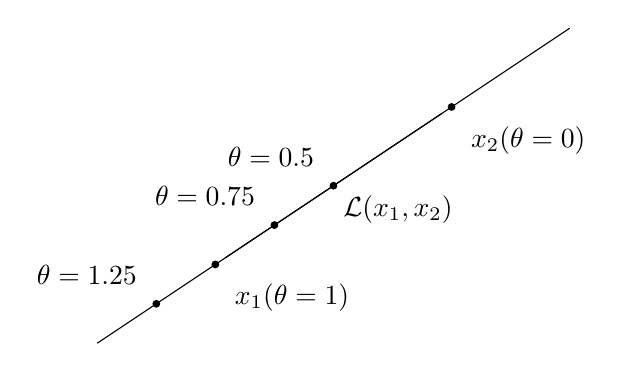
\begin{tikzpicture}
    \node[label = below right:{$x_1 (\theta = 1)$}] (A) at (0,0) {};
    \node at (A)[circle,fill,inner sep=1pt]{};
    \node[label = below right:{$x_2 (\theta = 0)$}] (B) at (3,2) {};
    \node at (B)[circle,fill,inner sep=1pt]{};
    \draw[] (A) -- (B) node[midway, below right] {$\mathcal{L}(x_1, x_2)$};
    \draw[] ($ (A)!-.5!(B) $) -- ($ (A)!1.5!(B) $);
    \node[label = above left:{$\theta = 0.5$}] (C) at ($ (A)!.5!(B) $) {};
    \node at (C)[circle,fill,inner sep=1pt]{};
    \node[label = above left:{$\theta = 0.75$}] (D) at ($ (A)!.25!(B) $) {};
    \node at (D)[circle,fill,inner sep=1pt]{};
    \node[label = above left:{$\theta = 1.25$}] (E) at ($ (A)!-.25!(B) $) {};
    \node at (E)[circle,fill,inner sep=1pt]{};
    \end{tikzpicture}
\end{figure}

如果令上述定义式中的$\theta \in [0,1]$,则称集合为$x_0$到$x_1$之间的线段。

\subsection{仿射集}
集合$C \subseteq \mathbb{R}^n$是仿射集当且仅当
$$\forall x_1,x_2 \in C, \exists \theta \in \mathbb{R}, x_0 = \theta x_1 + (1-\theta)x_2 \in C$$
这意味着仿射集包含其中任意向量的任意线性组合。在这里线性组合可以扩展的定义为$y = \sum_{i=1}^n a_i x_i$,其中$\sum_{i=1}^n a_i = 1$。

例如,线性方程组的解空间是一个仿射集。考虑方程组$Ax = b$,其中有$A\mathbb{R}^{m\times n}$以及$b\in\mathbb{R}^m$,则集合$C=\{x \in \mathbb{R}^n | Ax = b \}$是仿射集,因为对于任意的$x_1,x_2 \in C$,我们有$Ax_1 = b$和$Ax_2 = b$,则对于任意的$\theta \in \mathbb{R}$,有:

$$A(\theta x_1 + (1 - \theta)x_2) = \theta Ax_1 + (1 - \theta)Ax_2 = b$$

一个仿射集的平移仍然是仿射集。例如对一个仿射集$C$,定义其$x_0$平移集合为
$$V = C + x_0 = \{x-x_0 | x \in C\}$$
那么$V$仍是仿射集,因为对于任意的$x_1,x_2 \in V$,存在$x_1',x_2' \in C$使得$x_1 = x_1' + x_0$和$x_2 = x_2' + x_0$,则有:
$$\theta x_1 + (1 - \theta)x_2 = \theta (x_1' + x_0) + (1 - \theta)(x_2' + x_0) = \theta x_1' + (1 - \theta)x_2' + x_0$$
因此$\theta x_1 + (1 - \theta)x_2 \in V$


包含集合$C$中所有仿射组合的最小集合称为$C$的仿射包(affine hull),记为$\text{aff}(C)$。仿射包是一个仿射集,包含集合$C$中的所有点。

集合$C$的仿射维度定义为集合仿射包的维度。例如单位圆周$C = \{x \in \mathbb{R}^2 | \Vert x \Vert = 1\}$的仿射包为$\mathbb{R}^2$(显然圆周上任意不共线的三点的线性组合可以铺满整个二维平面),于是单位圆周的仿射维度为2。

定义集合$C$的内点集为:
$$\text{relint}(C) = \{x \in C |B(x,r)\cap \text{aff}(C) \subseteq C ,\exists r > 0\}$$
这里$B(x,r) = \{y| \| y-x \|  \leq r\}$,$\|\cdot\|$是任意范数(也就是距离度量)。

\subsection{凸集}

集合$C \subseteq \mathbb{R}^n$是凸集当且仅当对于任意的$x_1,x_2 \in C$,以及任意的$\theta \in [0,1]$,都有:
$$\theta x_1 + (1 - \theta)x_2 \in C,\quad \theta \in [0,1]$$
换句话说,就是集合中的任意点都能直接“看”到其它点。显然,一般仿射集都是凸集(因为其中包含了任意两点之间的线段)。

定义一般集合$C$的凸包为:
$$\text{conv}(C) = \{x \in \mathbb{R}^n | x = \sum_{i=1}^m \theta_i x_i ,\quad \sum_{i=1}^m \theta_i = 1 ,\quad \theta_i \geq 0 ,\quad x_i \in C\}$$
凸包是包含集合$C$的最小凸集。凸包的几何意义是将集合$C$中的所有点连接起来,形成一个凸(至少不凹)形状。

以上定义(凸集\&凸包)的有限和等式也可以推广为无限和等式甚至是黎曼积分的形式,只需要保证所有系数项求和结果为1即可。

\begin{figure}[htbp]
    \centering
    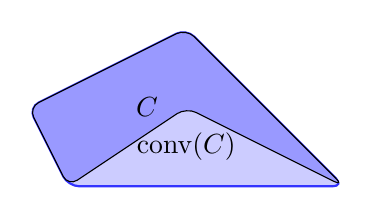
\begin{tikzpicture}
    \filldraw[draw=blue!80,fill=blue!20,thick,rounded corners] (1,1) -- (3,2) -- (5,0)--(1.5,0)--cycle;
    \filldraw[fill=blue!40,rounded corners] (1,1) -- (3,2) -- (5,0) -- (3,1) -- (1.5,0) --cycle;
    \node at (2.5,1) {$C$};
    \node at (3,0.5) {$\text{conv}(C)$};
    \end{tikzpicture}
\end{figure}

\subsection{锥体}
集合$C$是锥体(或称为非负齐次的)当且仅当对于任意的$x \in C$和任意的$\theta \geq 0$,都有$\theta x \in C$。也就是锥体中的任意点都可以被任意放大或缩小(只要缩小不为负数)。

集合$C$是凸锥体当且仅当它是锥体并且是凸集。也就是对于任意的$x_1,x_2 \in C$以及任意的$\theta_1,\theta_2 \geq 0$,都有:
$$\theta_1 x_1 + \theta_2 x_2 \in C$$

集合$C$的锥包定义为其中所有元素的“锥”组合,即$$\{\sum_{i=1}^k\theta_i x_i |x_c\in C ,\theta_i\geq 0\}$$

\begin{figure}[htbp]
    \centering
    \begin{tikzpicture}
    \filldraw[dashed,thin,draw=blue!80,fill=blue!20] (0,0)--(4,4)--(6,4)--(6,0) --cycle;
    \filldraw[draw=gray!80,fill=gray!20,thick,rounded corners] (1,1) -- (3,2) -- (5,0)--(1.5,0)--cycle;
    \filldraw[fill=gray!40,rounded corners] (1,1) -- (3,2) -- (5,0) -- (3,1) -- (1.5,0) --cycle;
    \draw[] (0,0) -- (4,4);
    \draw[] (0,0) -- (6,0);
    \node at (2.5,1) {$C$};
    \node at (3,0.5) {$\text{conv}(C)$};
    \node at (4,3) {$\text{锥包}(C)$};
    \node[below left] at (0,0) {$O$};
    \end{tikzpicture}
\end{figure}

\section{重要示例}
\subsection{简单凸集示例}
\begin{itemize}
    \item 空集$\emptyset$、单点集$\{x_0\}$、实空间$\mathbb{R}^n$
    \item 任何直线都是仿射集(也就是凸集),如果线段经过原点,则其还是凸锥
    \item 线段是凸集,但是不是仿射集
    \item 射线是凸集,如果其端点为原点则其还是凸锥
    \item 任意子空间都是仿射的,并且是凸锥
\end{itemize}
\subsection{超平面和半空间}
超平面是一个$n-1$维的仿射集,可以用一个线性方程来定义:
$$\{x \in \mathbb{R}^n | a^Tx = b\}$$
其中$a \in \mathbb{R}^n$,$b \in \mathbb{R}$。以上定义式可以移项获得另一种定义式:
$$\{x \in \mathbb{R}^n | a^T(x - x_0) = 0\}$$
其中$x_0$是超平面上任意一点,$a$是超平面的法向量(也就是垂直于超平面上所有向量的向量)。该定义式标明超平面由过$x_0$点的所有垂直于$a$的向量构成。

超平面将空间分为两部分,分别称为半空间。半空间是一个$n$维的凸集,可以给出一个(闭的)半空间的定义:
$$\{x \in \mathbb{R}^n | a^Tx \leq b\}$$
参考超平面的另一定义式,可以给出半空间的另一种定义式:
$$\{x \in \mathbb{R}^n | a^T(x-x_0) \leq 0\}$$
这个定义式代表的半空间是由所有与超平面法向量$a$夹角大于$90^\circ$的向量所组成的集合,也就是在超平面的“背面”上。

显然超平面是一个仿射集,并且是一个\textbf{凸集},其维度为$n-1$。半空间也是一个凸集,其维度为$n$。

\subsection{欧式球和椭球}

定义欧氏空间中的范数$\|\cdot\| : \|x\| = \sqrt{x^Tx}$。则在$\mathbb{R}^n$中欧式度量下的球体定义为
$$B(x_c,r)=\{x|\|x-x_c\|\leq r\} = \{x|(x-x_c)^T(x-x_c)\leq r^2\}$$
欧式球也有等价表述:
$$B(x_c,r)=\{x_c+ru|\|u\|\leq 1,u\in \mathbb{R}^n\}$$

欧式球是\textbf{凸集},因为对于任意的$x_1,x_2 \in B(x_c,r)$以及任意的$\theta \in [0,1]$,都有:
\begin{align*}
\| (\theta x_1 + (1 - \theta)x_2) - x_c \| &= \| \theta (x_1 - x_c) + (1 - \theta)(x_2 - x_c) \| \\
&\leq \theta \| x_1 - x_c \| + (1 - \theta)\| x_2 - x_c \| \\
&\leq \theta r + (1 - \theta)r = r
\end{align*}

从欧式球可以推广出椭球的概念。椭球是一个$n$维的\textbf{凸集},可以用一个二次型来定义:
$$E(x_c, A) = \{x \in \mathbb{R}^n | (x - x_c)^TA(x - x_c) \leq 1\}$$
其中$A$是一个对称正定矩阵,$x_c$是椭球的中心。(正定矩阵的定义是:对于任意的$x \in \mathbb{R}^n$,都有$x^TAx > 0$,并且$A$的特征值均为正数,对称即$P=P^T$)
也可以写为
$$\mathcal{E} = \{x_c+Au|\|u\|\leq 1\}$$
其中$A$是一个非奇异的方阵。

\subsection{范数球和范数锥}

对于$\mathbb{R}^n$中的任意范数$\|\cdot\|$,可以定义其范数球为:
$$B(x_c,r) = \{x \in \mathbb{R}^n| \|x-x_c\|\leq r\}$$
范数锥为
$$C=\{(x,t)\in \mathbb{R}^n \times \mathbb{R}|\|x\|\leq t\}\subseteq \mathbb{R}^{n+1}$$
显然以上二者都是\textbf{凸集}。

那么就有人要问了,老师老师,为什么这个锥它要多一个维度呢?其实原教材没有专门标注$(x,t)\in \mathbb{R}^n \times \mathbb{R}$,这里我写出来就是表达范数锥比原空间多了一个“高度”维度,分别在每个高度上的所有满足$\|x\|\leq t$的点构成整个锥体,可以想象锥体是不同高度的“层”拼接所得。例如二维向量的锥体就应该是一个三维图像。

特别的,定义欧式范数下的锥体,二阶锥体(Second-Order Cone,SOC)为:
$$\mathcal{Q} = \{(x,t) \in \mathbb{R}^{n+1} | (\sum_{i=1}^n x_i^2)^{\frac{1}{2}}\leq t\}$$
它被叫做二阶锥是因为它是由二次式定义而成的。

\subsection{多面体}

多面体可以定义为
$$\mathcal{P} = \{x|a_i^Tx\leq b_i, i=1,2,\ldots,m \text{且} c_j^Tx=d_j, j=1,2,\ldots,p \}$$
这个定义式标明多面体定义为$m$个半空间以及$p$个超平面的交集。直观上可以感受到,由若干个超平面围成的多面体是一个\textbf{凸集}。

定义式中半空间对应的超平面可以视作二维图形的“边”或者三维图形的“面”;其中的超平面(也就是等式条件)可以视作二维图形中的“截线”或者三维图形的“截面”。显然,线性无关的等式条件越多,最后得出的多面体的维度就越低。

例如在二维空间中,两个线性无关的等式条件(超平面)确定的多面体就只有一个点,三维空间中两个超平面加上一个半空间确定的多面体是一个线段或者一条射线。

\textbf{单纯形}是一类特殊的多面体,由$k+1$个仿射无关的点(也就是$k$个向量$v_1-v_0,\ldots,v_k-v_0$之间线性无关)定义。单纯形$C$的定义为:
$$C = \text{conv}\{v_0,v_1,\ldots,v_k\}$$

\subsection{半正定锥}

我们使用$S^n$来表示所有$n\times n$的对称矩阵的集合(这是一个$n(n+1)/2$维的向量空间),即
$$S^n=\{X\in\mathbb{R}^{n\times n}|X=X^T \}$$
定义半正定矩阵(对于任意的$x\in\mathbb{R}^n$,都有$x^TXx\geq 0$)
$$S^n_+ = \{X\in S^n|X\succeq 0\}$$
定义正定矩阵(对于任意的$x\in\mathbb{R}^n$,都有$x^TXx> 0$)$$S^n_{++} = \{X\in S^n|X\succ 0\}$$

以上定义式中,$\succeq$和$\succ$分别表示矩阵中的每个元素大于等于/大于0。这个符号表示偏序关系,具体定义将在后面“广义不等式”节中给出。

\section{保凸变换}
\subsection{交集}

凸集族在任意交运算下保持凸性(即使是无限的可列交乃至不可数交)。最简单的凸集交的例子是不同多面体的交,事实上多面体本身就是用多个半空间以及超平面的交定义的,在此基础上再加上更多半空间以及超平面的限制,最后得到的仍然是一个多面体(最严格的情况下得到$\emptyset$),仍然是凸集。

这一性质可以简单的理解,凸集中的所有元素都应当满足凸集成立的条件$\forall x_1,x_2 \in C,\quad\theta x_1 + (1 - \theta)x_2 \in C,\quad \theta \in [0,1]$,不同的凸集中的点都满足这个条件,许多凸集的交集中的点会满足每个凸集的限制,那么自然在这个交集中的点会满足凸集的要求。

相应的,并运算却不一定能保证凸性,例如说两个不同的单点集的并,是一个仅仅含有两个点的集合,显然不是凸集。这是因为并集中的点可能不满足其中某个集合的凸集要求,进而不满足整个集合的凸集要求。

\subsection{仿射变换}

凸集在仿射变换下仍然是凸集。仿射变换$f:\mathbb{R}^n\to\mathbb{R}^m,\quad f(x)=Ax+b$,其中$A\in\mathbb{R}^{m \times n}$和$b\in\mathbb{R}^m$。此时凸集$S$的象$f(S) = \{f(x)|x\in S\}$仍然是凸集,类似的,凸集$S$的逆象$f^{-1}(S) = \{x|f(x)\in S\}$仍然是凸集。

几个仿射变换简单的例子,经过以下变换后的结果集仍然为凸集。

\begin{itemize}
    \item 缩放变换($\alpha S = \{\alpha x | x\in S\}$)
    \item 平移变换($ S + a = \{x+a | x\in S\}$)
    \item 投影变换($T=\{x_1\in\mathbb{R}^m | (x_1,x_2)\in S \subseteq \mathbb{R}^{m\times n},\text{其中}x_2\in \mathbb{R}^n\}$)
    \item 加和变换($S_1+S_2= \{x_1+x_2 | x_1\in S_1,x_2\in S_2\}$)
    \item 笛卡尔积($S_1 \times S_2= \{(x_1,x_2) | x_1\in S_1,x_2\in S_2\}$)
    \item 部分和($S= \{(x_1+x_2,y )| (x_1,y)\in S_1,(x_2,y)\in S_2\}$)
\end{itemize}



\section{广义不等式}
\section{分离?和支撑超平面}
\section{对偶锥体和广义不等式}

\chapter{凸函数}
\chapter{凸优化问题}
\chapter{对偶性}

\part{应用}
\chapter{近似和拟合}
\chapter{统计估计}
\chapter{几何问题}
% 结束正文部分

% 参考文献
\bibliographystyle{plain}
\bibliography{references}

% 索引
\printindex

\end{document}